%!TEX root = ./presentation.tex
%&presentation.fmt

%!TEX root = ./presentation.tex 
\scrollmode

\documentclass[aspectratio=169]{beamer}
\usetheme{Madrid}


% -------------- COMPILE VARIABLES --------------
\newif\ifINTRO

\INTROfalse      % Build only intro slide


% ------------------ VARIABLES ------------------
\newcommand{\userName}{Pascal-Emmanuel Lachance}
\newcommand{\projectName}{PPPPP04}
\newcommand{\institution}{C3i}
\newcommand{\repo}{PPPPP}
\newcommand{\user}{raesangur}
\newcommand{\docName}{Presentation}

\author{\userName}
\title{\projectName}
\subtitle{Bonnes pratiques de design}
\institute{Compétitions de Conception de Circuits Imprimés}
\date{\today}


% ----------- CONFIGURATION INCLUDES ------------
%!TEX root = ../presentation.tex

%%%%%%%%%%%%
% PACKAGES %
%%%%%%%%%%%%

% =============== General Formatting ============
\usepackage[T1]{fontenc}
\usepackage{lmodern}
\usepackage{pifont}
\usepackage{amsmath}
\usepackage{amssymb}
\usepackage{fontawesome5}
\usepackage{comment}
\usepackage{adjustbox}
\usepackage{array}
\usepackage{multicol}
\usepackage{soul}
\usepackage[yyyymmdd]{datetime}
\usepackage{etoolbox}


% =============== Colors ============
\usepackage{colortbl}
\usepackage[many]{tcolorbox}
\usepackage{xcolor}
\usepackage{hyperref}

% =============== Math ============
\usepackage{mathtools}
\usepackage{nicefrac}
\usepackage{siunitx}
\usepackage{calc}

% =============== Tables ============
\usepackage{csvsimple}
\usepackage{makecell}
\usepackage{booktabs}

% =============== Figures ============
\usepackage{tikz}
\usepackage{circuitikz}
\usepackage{pgfplots}
\usepackage{animate}
\usepackage{environ}
\usepackage{caption}

% =============== Listings ============
\tcbuselibrary{listings}      % Raesangur
\usepackage{listings}         % Main package for inserting code
\tcbset{listing engine={listings}}
\usepackage[scaled]{beramono} % For using the beramono font

% =============== Bibliography ============
\usepackage[style=ieee,backend=biber]{biblatex}
\addbibresource{references.bib}

% =============== Package Setup ============
\newcolumntype{C}[1]{>{\centering\arraybackslash}p{#1}}

\renewcommand{\dateseparator}{--}

\newcommand{\cmark}{\ding{51}} % ✓
\newcommand{\xmark}{\ding{55}} % ✗

% =============== TiKz & PGF ============
\usetikzlibrary{arrows, shapes, calc, positioning, shadings, shadows.blur}
%\usetikzlibrary{external}
%\usepgfplotslibrary{external}
%\tikzexternalize
\pgfplotsset{compat=1.18}

% https://tex.stackexchange.com/a/539963/324686
% For title box shadow clippings
\makeatletter
\tikzset{
    reuse path/.code={\pgfsyssoftpath@setcurrentpath{#1}}
}
\makeatother
\tikzset{even odd clip/.code={\pgfseteorule},
    protect/.code={
        \clip[overlay,even odd clip,reuse path=#1]
        (-5383.99999pt,-5383.99999pt) rectangle (5383.99999pt,5383.99999pt);
}}

%!TEX root = ../presentation.tex


% -------------- BACKGROUNDS --------------

\newcommand\titlebackground {
    \usebackgroundtemplate{
    \begin{tikzpicture}[remember picture, overlay]
        \node[at=(current page.center)] {
            \includegraphics
            [width=\paperwidth, keepaspectratio]
            {pictures/background/background-PCB.png}
        };
    \end{tikzpicture}
    }
}


\newcommand\introbackground {
    \usebackgroundtemplate{
    \begin{tikzpicture}[remember picture, overlay]
        \node[at=(current page.center)] {
            \includegraphics
            [width=\paperwidth, keepaspectratio]
            {pictures/background/background-pcb-poster.png}
        };
    \end{tikzpicture}
    }
}

\newcommand\pausebackground {
    \usebackgroundtemplate{
    \begin{tikzpicture}[remember picture, overlay]
        \node[at=(current page.center)] {
            \includegraphics
            [height=\paperheight, keepaspectratio]
            {pictures/background/background-level-A.jpg}
        };
    \end{tikzpicture}
    }
}

\newcommand\chapterbackground {
    \usebackgroundtemplate{
    \begin{tikzpicture}[remember picture, overlay]
        \node[at=(current page.center)] {
            \includegraphics
            [width=\paperwidth, keepaspectratio]
            {pictures/background/background-level-B.jpg}
        };
    \end{tikzpicture}
    }
}

\newcommand\defaultbackground {
    \usebackgroundtemplate{
    \begin{tikzpicture}[remember picture, overlay]
        \node[at=(current page.center)] {
            \includegraphics
            [width=\paperwidth, keepaspectratio]
            {pictures/background/background-default.pdf}
        };
    \end{tikzpicture}
    }
}

\newcommand\pascalbackground {
    \usebackgroundtemplate{
    \begin{tikzpicture}[remember picture, overlay]
        \node[at=(current page.center)] {
            \includegraphics
            [width=\paperwidth, keepaspectratio]
            {pictures/background/background-pascal.pdf}
        };
    \end{tikzpicture}
    }
}

\newcommand\maxbackground {
    \usebackgroundtemplate{
    \begin{tikzpicture}[remember picture, overlay]
        \node[at=(current page.center)] {
            \includegraphics
            [width=\paperwidth, keepaspectratio]
            {pictures/background/background-max.pdf}
        };
    \end{tikzpicture}
    }
}

% -------------- TITLE PAGE --------------
\makeatletter
\setbeamertemplate{title page}
{
    \begin{columns}
        \begin{column}{0.75\textwidth}
            {
                \includegraphics[scale = 0.35]{pictures/logo/udes_logo.pdf}\\
            }
            \vspace{24pt}
            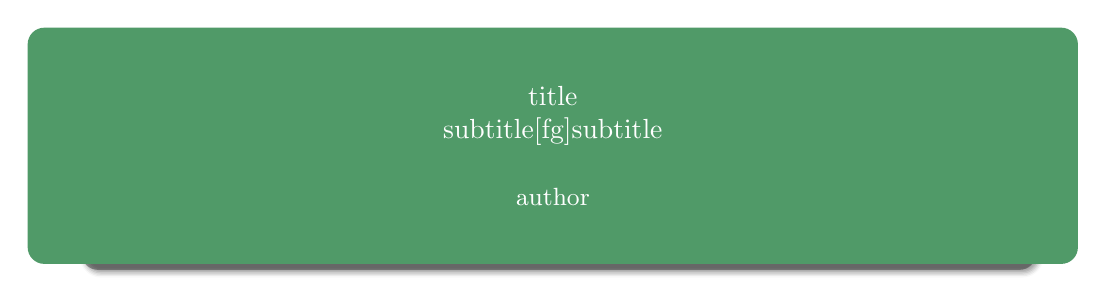
\begin{tikzpicture}
                \def\boxwidth{\textwidth}
                \def\boxheight{3cm}
                \def\cornerradius{6pt}
                \def\shadowshift{0.5ex}
                
                \node[fill=UDSgreenSolidarite,
                      fill opacity=0.9,
                      rounded corners=6pt,
                      minimum width=1.1\boxwidth, minimum height=\boxheight,
                      text=white,
                      text opacity=1,
                      align=center] (mainbox) at (0, 0){
                    \usebeamerfont{title}
                    \textbf{\inserttitle}\\
                    \usebeamerfont{subtitle}\usebeamercolor[fg]{subtitle}
                    \textbf{\insertsubtitle}\\\\
                    \small\usebeamerfont{author}\insertauthor
                };

                \path (mainbox) node[rectangle, minimum width=1.0999\boxwidth, minimum height=0.996*\boxheight, rounded corners=\cornerradius, save path=\inbox] at (0, 0) {};
                \tikzset{protect=\inbox}

                \begin{scope}[transparency group, opacity=1]
                    \fill[color=black, opacity=0.33, rounded corners=\cornerradius,
                          blur shadow = {shadow xshift=.25ex, shadow yshift=-.25ex}]
                        (-0.5\boxwidth + \shadowshift, 0.5*\boxheight - \shadowshift) rectangle 
                        (0.5\boxwidth + \shadowshift, -0.5*\boxheight - \shadowshift);
                \end{scope}
            \end{tikzpicture}
            \vspace{24pt}
        \end{column}
        \begin{column}{0.25\textwidth}
        \end{column}
    \end{columns}
}
\makeatother


\newcommand\thankyouframe{
    \begin{frame}
    \begin{multicols}{2}
        \begin{beamercolorbox}[sep=8pt, center, shadow=true, rounded=true, wd=0.5\textwidth, bgopacity=0.85]{title}
            \usebeamerfont{title}Merci!\\
        \end{beamercolorbox}%
    \vfill\null
    \columnbreak
    \end{multicols}
\end{frame}
}

%!TEX root = ../presentation.tex



% Insert a figure with optional scaling and caption.
% 1: Width as a fraction of \textwidth   (default: 1)
% 2: Height as a fraction of \textheight (default: 0.8)
% 3: Caption text (optional)
% 4: Filename of the image (relative to 'pictures/' directory, no extension needed)
%
% Example:
% \makefigure[0.9][0.5][A sample image]{example-image}
\NewDocumentCommand{\makefigure}{O{1} O{0.8} o m}{%
    \begin{figure}%
        \centering%
        \includegraphics%
            [width=#1\textwidth, height=#2\textheight, keepaspectratio, page=1]%
            {pictures/#4}%
        \IfValueTF{#3}{%
            \caption*{#3}%
        }{}%
    \end{figure}%
}


% Insert a figure with border and with optional scaling and caption.
% 1: Width as a fraction of \textwidth   (default: 1)
% 2: Height as a fraction of \textheight (default: 0.8)
% 3: Caption text (optional)
% 4: Filename of the image (relative to 'pictures/' directory, no extension needed)
%
% Example:
% \makefigureborder[0.75][0.7][A sample image]{example-image}
\NewDocumentCommand{\makefigureborder}{O{1} O{0.8} o m}{%
    \begin{figure}%
        \centering%
        \tcbox[colframe=accent, colback=background]{
            \includegraphics%
                [width=#1\textwidth, height=#2\textheight, keepaspectratio, page=1]%
                {pictures/#4}%
            \IfValueTF{#3}{%
                \caption*{#3}%
            }{}%
        }
    \end{figure}%
}


% Create a TikZ circuit figure with adjustable size.
% 1: Width as a fraction of \textwidth   (default: 1)
% 2: Height as a fraction of \textheight (default: 0.8)
%
% Example:
% \begin{maketikzfigure}[0.7][0.5]
%     \draw (0,0) to[battery] (0,2);
% \end{maketikzfigure}
\NewDocumentEnvironment{maketikzfigure}{O{1} O{0.8}}{%
    \vspace{-16pt}%
    \begin{center}%
        \begin{adjustbox}{width=#1\textwidth, height=#2\textheight, keepaspectratio}%
            \begin{circuitikz}[american voltages, american currents]%
}
{%
            \end{circuitikz}%
        \end{adjustbox}%
    \end{center}%
}




% Begin a two-column layout with adjustable left column width.
% 1: Width of the left column as a fraction of \textwidth (default: 0.5)
%    The right column will take the remaining space after the left column
%
% Example:
% \begin{twocolumns}[0.6]
%   \leftcol
%     Left side content.
%   \rightcol
%     Right side content.
% \end{twocolumns}
\NewDocumentEnvironment{twocolumns}{O{0.5}}{%  
  \def\leftcolwidth{#1\textwidth}%
  \def\rightcolwidth{\dimexpr \textwidth - #1\textwidth\relax}%
  
  \begin{columns}%
}{%
  \end{column}%
  \end{columns}%
}

\NewDocumentCommand{\leftcol}{}{%
  \begin{column}{\leftcolwidth}%
}

\NewDocumentCommand{\rightcol}{}{%
  \end{column}%
  \begin{column}{\rightcolwidth}%
}


% Color an icon
% 1: Color name   (optional, default: accent)
% 2: Icon command (e.g., \faCheck)
%
% Example:
% \icon{\faCheck}
% \icon[red]{\faTimes}
\newcommand{\icon}    [2][accent] {\textcolor{#1}{#2}}

% Display an icon at the start of a list item with customizable color and spacing.
% 1: Color name       (optional, default: accent)
% 2: Horizontal space (optional, default: -12pt)
% 3: Icon command     (e.g., \faCheck)
%
% Example:
% \item[] \itemicon           {\faCheck}
% \item[] \itemicon[gray]     {\faCircle}
% \item[] \itemicon[red][-6pt]{\faTimes}
\NewDocumentCommand{\itemicon}{O{accent} O{-12pt} m}{\hspace{#2}\icon[#1]{#3}}



% Create a two-column list using a tabular environment.
% 1: Font size or formatting command (optional, default: \normalsize)
% 2: Row spacing via \arraystretch   (optional, default: 1.25)
% 3: Tabular column format           (optional, default: c l)
%
% Example:
% \begin{makelist}[\small][1.5]
%   \icon{\faCheck} & Item one \\
%   \icon{\faTimes} & Item two \\
% \end{makelist}
\NewDocumentEnvironment{makelist}{O{\normalsize} O{1.25} O{c l}}{%
    #1%
    \renewcommand{\arraystretch}{#2}%
    \begin{tabular}{#3}%
}{%
    \end{tabular}%
    \renewcommand{\arraystretch}{1}%
}


%Roman Numerals
\makeatletter
\newcommand*{\rom}[1]{\expandafter\@slowromancap\romannumeral #1@}
\makeatother


% Insert a table from the tables folder. This Table can be automatically
% generated from a dataframe in Pandas using pd.DataFrame().to_latex()
% 1: name of the table file         (without .tex extension)
% 2: caption                        (optional, defaults to none)
% 3: label                          (optional, auto-generated from table name if omitted)
% 4: placement                      (optional, defaults to 'htbp')
%
% Usage:
%   \maketable{table1}
%   \maketable{table1}{My caption}
%   \maketable{table1}{My caption}{tab:mylabel}
%   \maketable{table1}{My caption}{tab:mylabel}[H]

\NewDocumentCommand{\maketable}{m o o o}{%
    \begin{table}[{#4}]%
    \centering
    \IfValueT{#2}{\caption{#2}}%
    \IfValueTF{#3}{\label{#3}}{\label{tab:#1}}%
    \input{tables/#1.tex}%
    \end{table}%
}
%!TEX root = ../presentation.tex

% =============== Colors ============
\definecolor{UDSgreenDurable}{RGB}{149, 193, 78}
\definecolor{UDSgreenVivacite}{RGB}{121, 181, 81}
\definecolor{UDSgreenCreativite}{RGB}{90, 173, 85}
\definecolor{UDSgreenFierte}{RGB}{0, 167, 89}
\definecolor{UDSgreenSolidarite}{RGB}{61, 143, 88}
\definecolor{UDSgreenSolidariteDark}{RGB}{0, 120, 25}
\definecolor{UDSgreenBienEtre}{RGB}{68, 124, 90}
\definecolor{UDSgreenReussite}{RGB}{72, 106, 92} 
\definecolor{UDSgrey}{RGB}{228, 232, 225} 
\definecolor{UDSdarkGrey}{RGB}{15, 42, 18} 
\definecolor{UDSdarkGrey2}{RGB}{55, 82, 58} 

\setbeamercolor{palette primary}{bg=UDSgreenSolidarite,fg=white}
\setbeamercolor{palette secondary}{bg=UDSgreenFierte,fg=white}
\setbeamercolor{palette tertiary}{bg=UDSgreenCreativite,fg=white}
\setbeamercolor{palette quaternary}{bg=UDSgreenReussite,fg=white}
\setbeamercolor{structure}{fg=UDSgreenReussite} % itemize, enumerate, etc
\setbeamercolor{section in toc}{fg=UDSgreenBienEtre} % TOC sections
\setbeamercolor{section in toc shaded}{fg=UDSdarkGrey}
\setbeamercolor{background canvas}{bg=UDSgrey}


\colorlet{foreground}{black}
\colorlet{background}{UDSgrey}
\colorlet{header}{UDSgreenSolidariteDark}
\colorlet{accent}{UDSgreenFierte}
\colorlet{accent2}{red}



% =============== Math ===============
\sisetup{
  per-mode=fraction,
  fraction-function=\nicefrac,
  detect-weight=true,
  detect-family=true
}

\DeclareSIUnit\bit{b}
\DeclareSIUnit\bits{bits}
\DeclareSIUnit\dbm{dBm}
\DeclareSIUnit\baud{baud}
\DeclareSIUnit\mil{mil}
\DeclareSIUnit\inch{in}


%!TEX root = ../presentation.tex


% ----------------- INLINE CODE -----------------

% Display monospace text in a grey box. Similar to ` text in markdown.
% 1: Color of the text in the textbox - default: [black]
% 2: Text to display
%
% Note: This command sometimes continues in the margins of the page, 
% putting the punctuation as the 3rd argument prevents the following punctuation
% to be alone at the start of the next line.
%
% Example:
% This is an \inline{example} without a specified color.
% This is another \href{https://www.example.com}{\inline[blue]{example}}
\newcommand{\inline}[2][black]{ %
  \hspace{-8pt}%
  \begingroup%
  \raggedright%
  {
    \mbox{%
      \raggedright\tcbox[on line,%
                         boxsep=4pt, left=-1pt,right=-1pt,top=-4pt,bottom=-4.5pt,%
                         opacityframe=0, colback=gray!50,%
                         fontupper={\strut},%
                         enhanced, breakable]%
      {%
        \raggedright\lstinline[basicstyle=\ttfamily\small\color{#1},%
                               breaklines=true, breakatwhitespace=true,%
                               moredelim={[s][\ttfamily]{_}{_}}]%
      {#2}%
      }%
    }%
  }
  \endgroup%
  \hspace*{-8pt}~%
}


% --------------- REGULAR LISTING ---------------

% Create a lstlisting environment with custom syntax highlighting.
% 1: Syntax highlighting language - default: [logbook]
% 
% Note: The syntax highlighting argument is currently unused, as no other styles than logbook have been defined.
%
% Example:
% \begin{makelisting}{python}
% if __name__ == "__main__":
%     print("Example")
% \end{makelisting}
\lstnewenvironment{makelisting}[2][]
{
  \vspace{-8pt}
  \lstset{style=logbook #1}
}
{
  \vspace{-12pt}
}

% Create two aligned columns with proper spacing.
% Used to compare two listings or figures easily.
%
% Example:
% \begin{makecompare}
%   This is the first example, on the left.
%   \newcol
%   This second example is on the right!
% \end{makecompare}
\newenvironment{makecompare}
{
  \vspace{-1.25\cringlineskip}
  \begin{multicols}{2}
}
{
  \end{multicols}
  \vspace{-2\cringlineskip}
}


 % ----------------- CODE BLOCK -----------------
% https://tex.stackexchange.com/a/468526
\newtcbinputlisting[auto counter, list inside = lol, list type = {lstlisting}]{\makecode}[3][logbook]{
  breakable,
  listing file = {code/#3},
  listing options={style = logbook},
  listing only,
  boxrule = 1pt,
  title = {\textbf{Code \thetcbcounter:} \textbf{#2} \hfill \textbf{#3}},
  label = code:#3
}


% ---------------- CODE FORMATS -----------------
\lstdefinestyle{logbook}{
  escapeinside={<@}{@>},
  language=C,
  aboveskip=0.5cm,
  breakatwhitespace=false,
  breaklines=true,
  numbers=left,
  numbersep=8pt,
  numberfirstline = false,
  linewidth=\textwidth,
  stepnumber=1,
  frame=lines,
  framesep=0pt,
  framerule=0pt,
  framextopmargin=3pt,
  framexbottommargin=3pt,
  framexleftmargin=0.4cm,
  xleftmargin={0.75cm},
  rulecolor=\color{Black},
  rulesep=.4pt,
  %backgroundcolor=\color{background},
  basicstyle=\small\ttfamily,
  identifierstyle=\color{RoyalBlue},
  commentstyle=\color{ForestGreen}\itshape,
  keywordstyle=\color{Plum}\bfseries,
  numberstyle=\small\ttfamily,
  stringstyle=\ttfamily\color{RedOrange},
  showstringspaces=false,
  showspaces=false,
  keepspaces=true,
  showtabs=false,
  tabsize=4,
  captionpos=t,
}

%\input{config/presentation-bibliography}
%!TEX root = ../presentation.tex 


\makeatletter
\let\slideno\beamer@slideinframe
\makeatother

\setbeamertemplate{caption}[numbered]


% Remove nagivation symbols for intro frame generation
\ifINTRO
    \includeonlyframes{intro}
    \setbeamertemplate{navigation symbols}{}
\fi


% -------------- ITEMS --------------

\setbeamertemplate{itemize item}{\large$\bullet$}
\setbeamertemplate{itemize subitem}{\small$\bullet$}
\setbeamertemplate{itemize subsubitem}{\tiny$\bullet$}

\makeatletter
\setbeamertemplate{section in toc}{%
    \begin{raggedright}%
      \leavevmode%
      \hspace{1em}%
      \Large{$\bullet$}%
      \hspace{0.5em}%
      \large{\inserttocsection}\par%
    \end{raggedright}%
}
\makeatother
\makeatletter
\setbeamertemplate{subsection in toc}{%
    \begin{raggedright}%
      \leavevmode%
      \hspace{3em}%
      \large{$\bullet$}%
      \hspace{0.5em}%
      \normalsize{\inserttocsubsection}\par%
    \end{raggedright}%
}
\makeatother

\makeatletter
\patchcmd{\beamer@sectionintoc}{\vskip1.5em}{\vskip1em}{}{}
\makeatother


\usebeamertemplate{mytheme}

% -------------- TABLE OF CONTENT --------------

\newcommand\maketoctitleheader{
    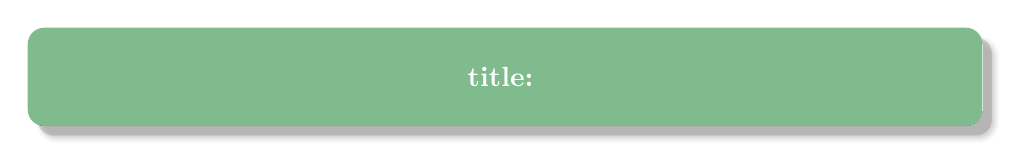
\begin{tikzpicture}
        \def\boxwidth{\linewidth}
        \def\boxheight{1.25cm}
        \def\cornerradius{6pt}
        \def\shadowshift{0.8ex}
        
        \node[fill=header,
              fill opacity=0.5,
              rounded corners=6pt,
              minimum width=\linewidth, minimum height=1.25cm,
              text=white,
              text opacity=1,
              align=center] (mainbox) at (0, 0)
        {\textbf{\usebeamerfont{title}\insertsectionhead:\;\insertsection}};

        \path (mainbox) node[rectangle, minimum width=\boxwidth, minimum height=0.989*\boxheight, rounded corners=\cornerradius, save path=\inbox] at (0, 0) {};
        \tikzset{protect=\inbox}

        \begin{scope}[transparency group, opacity=0.5]
            \fill[color=black, opacity=0.3, rounded corners=\cornerradius, blur shadow = {shadow xshift=.25ex, shadow yshift=-.25ex}] 
                (-0.5\boxwidth + \shadowshift, 0.5*\boxheight - \shadowshift) rectangle 
                (0.5\boxwidth + \shadowshift, -0.5*\boxheight - \shadowshift);
        \end{scope}
    \end{tikzpicture}
}



\newcommand\maketoc{%
    \AtBeginSection[]{%
        \icebergbackground%  <-- set the shifted background
        \begin{frame}[plain]%
            \vfill%
            \centering%
            \maketoctitleheader%
            \vfill%
        \RightSideTOC%
         
    \end{frame}
    \defaultbackground
    }
%    \AtBeginSection[]{%
%        \defaultbackground%
%        \begin{frame}[plain]%
%            \vfill%
%            \centering%
%            \maketoctitleheader%
%            \vfill%
%            \tableofcontents[currentsection, hideothersubsections]%
%            \vfill%
%      \end{frame}%
%    }%

    \AtBeginSubsection[]{%
        \icebergbackground%
        \begin{frame}[plain]%
            \vfill%
            \centering%
            \maketoctitleheader%
            \vfill%
            \tableofcontents[currentsection, currentsubsection, subsectionstyle=show/shaded/hide]%
            \vfill%
        \end{frame}%
        \defaultbackground
    }%
}%


% -------------- HEADER AND FOOTER --------------


\defbeamertemplate*{frametitle}{mytheme}{%
  \vspace{0cm}%
  {\usebeamerfont{title}\usebeamercolor[bg]{title}%
    \ifdefempty{\insertsubsectionhead}%
        {% No subsection → use section title
        \underline{\insertsectionhead:\;\insertsection}\;--\;\insertframetitle
        }%
        {% Subsection exists -> use subsection
        {\color{black}[\insertsubsectionhead]}\;\underline{\insertsectionhead:\;\insertsubsection}\;--\;\insertframetitle
        }%
    }\\[-0.55cm]%
    \hfill%
    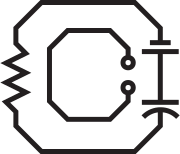
\includegraphics[height=0.635cm]{pictures/logo/c3i.pdf}%
    \hspace{0.25cm}%
    \includegraphics[height=0.635cm]{pictures/logo/m1_alpha.pdf}\par
    \vspace{-0.3cm}%
    \textcolor{UDSgreenSolidarite}{%
    \noindent\rule{\textwidth}{1pt}%
  }%
}

\defbeamertemplate*{footline}{mytheme}{%
    \leavevmode%
    \hbox{%
        \begin{beamercolorbox}%
            [wd=.33\paperwidth, ht=2.25ex, dp=1ex, center]{author in head/foot}%
            \usebeamerfont{author in head/foot}%
                \initials
        \end{beamercolorbox}%
        \begin{beamercolorbox}%
            [wd=.34\paperwidth, ht=2.25ex, dp=1ex, center]%
            {title in head/foot}%
            \usebeamerfont{title in head/foot}%
                \textbf{\inserttitle}%
        \end{beamercolorbox}%
    }%
    \begin{beamercolorbox}%
        [wd=.33\paperwidth, ht=2.25ex, dp=1ex, right]%
        {date in head/foot}%
        \hfill\usebeamerfont{date in head/foot}%
            \today{}%
        \hfill%
        \insertframenumber{} / \inserttotalframenumber%
        \hspace*{2ex}%
    \end{beamercolorbox}%
}%





% --------------- BUILD SETTINGS ----------------
\pdfcompresslevel=1
\pdfobjcompresslevel=1

% \tikzexternalize

% \dump
\csname endofdump\endcsname
\endofdump
%mylatex




% ----------------------- BEGIN DOCUMENT ------------------------

\begin{document}

\titlebackground

\begin{frame}[plain]
    \maketitle
\end{frame}

\introbackground

\begin{frame}[plain, label=intro]
    \centering
    \Large

    \textcolor{white}{
        \LARGE{\textbf{\inserttitle}}\\
        \textbf{\textit{\insertsubtitle}}\\
        Par: \insertauthor\\
    }
    \vspace{24pt}
    \begin{tabular}{c l}
        \textcolor{UDSgreenFierte}{\faShield*}
            & \textcolor{white}{~Comment protéger une alimentation?}\\
            [0.3em]
        \textcolor{UDSgreenFierte}{\faSlidersH}
            & \textcolor{white}{~Quels sont les types de régulateurs?}\\
            [0.3em]
        \textcolor{UDSgreenFierte}{\faEquals}
            & \textcolor{white}{~À quoi sert le découplage?}\\
            [0.3em]
        \textcolor{UDSgreenFierte}{\faWaveSquare}
            & \textcolor{white}{~Comment filtrer une alimentation?}\\
            [0.3em]
        \textcolor{UDSgreenFierte}{\faProjectDiagram}
            & \textcolor{white}{~Comment conçevoir un arbre d'alimentation?}\\
    \end{tabular}
\end{frame}



% - TOC -
\maketoc

% ------------ SECTIONS -----------

\defaultbackground
%!TEX root = ../presentation.tex 

\section{Bonnes pratiques non-classées}

\section{Définition des besoins}
% Volume, reliability, test
% Envisager la complexité
% Pareto
% - 80% de ton power 20% des pièces
% - 80% des coûts 20% des pièces
% - 80% du temps de design sur 20% du design
% - 20% des efforts pour 80% des résultats
% Faire des schéma-blocs
% - Général
% - Power Delivery Network
% - MCU / FPGA
% - Flow de communication


\section{Debugging}
% Toujours avoir plusieurs méthodes de debug
% Être conscient des outils de debug à ta disposition
% Si tu as un problème ici, comment tu debug

\section{Simulation}

%!TEX root = ../presentation.tex 


\section{Bonnes pratiques des composantes \& BOM}

\subsection{Footprints}
% Toujours valider les footprints
% Faire tes footprints toi-même
% Faire très attention aux transistors!
% Marqueurs de pin 1
% Modèle 3D pour toutes les pièces
% S'assurer de respecter les couches mécaniques

\subsection{Symboles}
% Faire les symboles toi-même
% Utiliser les informations de pin (Input / Output / Passive / Power)
% Input à gauche, output à droite

\subsection{Datasheets}
% Lis la datasheet au complet!
% Lire les schematics des evaluation boards
% Lire les application notes faites par les fabricants de pièces
%  - Application notes sur le board design
% Toujours valider les courbes de power
%  - Combien de courant est-ce que la chip va prendre?
% Manufacturier donne parfois des configurateurs
% Valider les plages de température, de tension
%  - Comment le chip va chauffer dans ton utilisation?

\subsection{Recherche de pièces}
% Comment browser Digikey, Mouser, LCSC
%  - Marketplace components sur Digikey
% Not recommended for new designs
%  - Aller sur le site du manufacturier
% Liste de fournisseurs
%  - Carte du monde
%  - Attention aux tarrifs
%  - Attention aux fausses pièces

\subsection{BOM}
% Faire valider le BOM par quelqu'un d'autre
% Consolidation du BOM
% Un assemblage va coûter autant que les pièces
% Prix de vente = Fab price * 2.5 (eevblog)
% Limiter la taille du BOM (assemblage)
% Toujours tout mettre dans le BOM
%  - Fusibles
%  - Vis & Mechanical
%  - Alimentations
%!TEX root = ../main.tex 

\section{Bonnes pratiques de schéma}

\subsection{Clareté}
% Éviter tous les croisements, pas de GND dans les airs, aligner
% Utiliser la grille
% Utiliser des net names
% Quand utiliser des net locaux, globaux, power
% Inputs à gauche, output à droite
% Garder les sections modulaires, bien indiquer les sections
% Tout devrait être dans le schematics
%  - Mettre plus que pas assez
%  - Notes pour le programmeur, pour le layouteur, pour l'assembleur
%  - Tu ne devrais pas avoir à réouvrir une datasheet
% Mettre des couleurs sur les nets
% Utiliser des net classes

\subsection{Notes}
% Mettre un schéma-bloc et un arbre d'alimentation
%     Draw.io
%     Travailler en hiérarchique
% Calculer le power pour chaque bloc et page
% Mettre des notes avec tous les calculs
% Mettre des notes avec pages de datasheets
% Mettre les courbes d'efficacité etc.
% Cartouche
% Indiquer les tailles et tolérances de composantes sur le schematic
% Notes pour les pins
% - Qu'est-ce qu'elles font, comment configurer

\subsection{Testpoints et Debugging}
% Valider les boot sequences & power-sequence
% Se servir des pins flottantes
%  - Ajouter IO, LED, Testpoint, UART
% Mettre des systèmes de mesure de courant
% Met toujours plus de testpoints qu'on pense
%  - Différents types de testpoints

\subsection{Outils}
% Passer le DRC
% Les 0R sont tes amis
%  - Peut remplacer une ferrite ou une shunt
%  - Pins EN et CFG
%  - Solder Bridge Pads

\subsection{Autre}
% Bien faire son découplage
% Toujours mettre des protections
%  - ESD
%  - Power
% Export ton schematic en PDF pour l'ouvrir sans logiciel

%!TEX root = ../main.tex 

\section{Comment conçevoir un arbre d'alimentation?}

\subsection{Déterminer les besoins}

\begin{frame}{Tensions d'opération}
    \begin{itemize}
        \item[] \textcolor{UDSgreenFierte}{\faToggleOn} ~Chaque puce a une tension d'opération
        \item[] \textcolor{UDSgreenFierte}{\faList} ~Parfois plusieurs tensions possible ($\SI{3.3}{\volt}$ jusqu'à $\SI{5}{\volt}$)
        \item[] \textcolor{UDSgreenFierte}{\faSignal} ~Parfois plusieurs tensions nécessaires!
        \bigskip
        \item[] \textcolor{UDSgreenFierte}{\faWaveSquare} ~Parfois les puces peuvent avoir des IO à des tensions différentes
    \end{itemize}
\end{frame}

\begin{frame}{Courant d'opération}
    \begin{columns}
        \only<2> {
            \begin{column}{0.55\textwidth}
        }
        \only<1, 3> {
            \begin{column}{0.66\textwidth}
        }
            \begin{itemize}
                \item[] \icon{\faListOl} ~Pour chaque puce, à ses tension d'opération, récupérer:
                \begin{itemize}
                    \item[] \itemicon{\faBed}
                        ~Le courant minimal (sleep)
                    \item[] \itemicon{\faWalking}
                        ~Le courant normal d'opération
                    \item[] \itemicon{\faRunning}
                        ~Le courant maximal d'opération
                    \item[] \itemicon{\faEquals}
                        ~Parfois tout le même
                \end{itemize}
                \only<2-> {
                    \item[] \itemicon[accent][-6pt]{\faArrowRight}
                        ~Conçevoir circuit pour pouvoir passer le courant maximal
                    \item[] \itemicon[accent][-6pt]{\faChartLine}
                        ~Choisir régulateurs pour avoir efficacité maximale au courant nominal
                }
                \only<3> {
                    \item[] \itemicon[accent][-6pt]{\faList} ~Aussi rassembler tous les courants autres
                    \begin{itemize}
                        \item[] \itemicon{\faSync}
                            ~Moteurs
                        \item[] \itemicon{\faLightbulb}
                            ~LEDs et affichage
                        \item[] \itemicon{\faEthernet}
                            ~Connecteurs et sous-cartes
                    \end{itemize}
                }
            \end{itemize}
        \end{column}
        
        \only<2> {
        \begin{column}{0.45\textwidth}
            \begin{figure}
                \includegraphics<2>[width=\textwidth, height=0.75\textheight, keepaspectratio]{pictures/switching-efficiency-curve.png}
            \end{figure}
        \end{column}
        }
        \only<1, 3> {
        \begin{column}{0.33\textwidth}
            \begin{figure}
                \includegraphics<3>[width=\textwidth, height=0.75\textheight, keepaspectratio]{pictures/switching-efficiency-curve.png}
            \end{figure}
        \end{column}
        }
    \end{columns}
\end{frame}

\begin{frame}{Trouver le courant d'opération}
    \begin{figure}
        \includegraphics[width=\textwidth, height=0.75\textheight, keepaspectratio]{pictures/ad4050-power.png}
    \end{figure}
    \href{https://www.analog.com/media/en/technical-documentation/data-sheets/ad4050-ad4056.pdf}{Analog Devices - AD4050 - 12-Bit 2MSPS SAR ADC}
\end{frame}

\begin{frame}{Besoins en stabilité}
    \begin{itemize}
        \item[] \textcolor{UDSgreenFierte}{\faWater} ~Déterminer les besoins de chaque puce en stabilité
        \item[] \textcolor{UDSgreenFierte}{\faBatteryQuarter} ~Quel est le $\Delta V$ maximum tolérable pour l'opération de la puce
        \item[] \textcolor{UDSgreenFierte}{\faTachometer*} ~Quelle est la précision nécessaire pour une puce analogique
        \item[] \textcolor{UDSgreenFierte}{\faClock} ~À quel point un $\Delta V$ peut introduire un $\Delta f$ pour la fréquence?
    \end{itemize}

    \begin{columns}
        \begin{column}{0.5\textwidth}
            \only<2-> {
            \begin{itemize}
                \item[] \textcolor{UDSgreenFierte}{\faChartBar} ~Toujours mieux de quantifier
                \item[] \textcolor{UDSgreenFierte}{\faList} ~\textbf{Permet de déterminer type de régulateur}
            \end{itemize}
            }
        \end{column}
        \begin{column}{0.5\textwidth}
            \begin{figure}
                \includegraphics[width=\textwidth, height=0.45\textheight, keepaspectratio]{pictures/eye-diagram.png}
            \end{figure}
        \end{column}
    \end{columns}
\end{frame}


\subsection{Bilan d'alimentation}

\begin{frame}{Bilan d'alimentation - Example - Alimentation 12V}
    \centering
    \Large
    \renewcommand{\arraystretch}{1.2}
    \vspace{-6pt}

    \begin{tabular}{>{\color{UDSgreenSolidarite}}c l | l | l | l | l | l}
    \rowcolor{UDSgreenSolidarite}
    & \textcolor{white}{\textbf{IC}}
    & \textcolor{white}{\textbf{Tension}}
    & \textcolor{white}{\textbf{I min}}
    & \textcolor{white}{\textbf{I nom}}
    & \textcolor{white}{\textbf{I max}} 
    & \textcolor{white}{\textbf{Type}}\\
    \hline
    \textcolor{UDSgreenFierte}{\faMicrochip} &
        \textbf{IC 1} &
        $\SI{3.3}{\volt}$ &
        $\SI{10}{\micro\ampere}$ &
        $\SI{17.5}{\milli\ampere}$ &
        $\SI{17.5}{\milli\ampere}$ &
        Digital\\
    \textcolor{UDSgreenFierte}{\faMicrochip} &
        \textbf{IC 2} &
        $\SI{3.3}{\volt}$ &
        $\SI{10}{\milli\ampere}$ &
        $\SI{10}{\milli\ampere}$ &
        $\SI{10}{\milli\ampere}$ &
        Digital\\
    & \hspace{16pt}\raisebox{10pt}{\rotatebox{-90}{\faLevelUp*}} &
        $\SI{3.3}{\volt}$ &
        $\SI{0}{\micro\ampere}$ &
        $\SI{10}{\milli\ampere}$ &
        $\SI{50}{\milli\ampere}$ &
        Analog\\
    \textcolor{UDSgreenFierte}{\faMicrochip} &
        \textbf{IC 3} &
        $\SI{2.5}{\volt}$ &
        $\SI{20}{\milli\ampere}$ &
        $\SI{20}{\milli\ampere}$ &
        $\SI{50}{\milli\ampere}$ &
        Analog\\
    \textcolor{UDSgreenFierte}{\faLightbulb} &
        \textbf{LEDs} &
        $\SI{5}{\volt}$ &
        $\SI{0}{\ampere}$ &
        $\SI{80}{\milli\ampere}$ &
        $\SI{80}{\milli\ampere}$ &
        Digital\\
    \textcolor{UDSgreenFierte}{\faUsb} &
        \textbf{USB} &
        $\SI{5}{\volt}$ &
        $\SI{0}{\ampere}$ &
        $\SI{100}{\milli\ampere}$ &
        $\SI{500}{\milli\ampere}$ &
        Digital\\
    \textcolor{UDSgreenFierte}{\faFan} &
        \textbf{Stepper} &
        $\SI{12}{\volt}$ &
        $\SI{0}{\ampere}$ &
        $\SI{300}{\milli\ampere}$ &
        $\SI{750}{\milli\ampere}$ &
        Digital\\
    \hline
    \textcolor{UDSgreenFierte}{\boldmath$\Sigma$} & \textbf{Total} & &
        \textbf{\boldmath$\SI{30.01}{\milli\ampere}$} &
        \textbf{\boldmath$\SI{537.5}{\milli\ampere}$} &
        \textbf{\boldmath$\SI{1457.5}{\milli\ampere}$} & \\
    \end{tabular}
\end{frame}

\begin{frame}{Bilan d'alimentation - Example - Alimentation 12V}
    \centering
    \Large
    \renewcommand{\arraystretch}{1.2}
    \vspace{-6pt}

    \begin{tabular}{>{\color{UDSgreenSolidarite}}c l | l | l | l}
    \rowcolor{UDSgreenSolidarite}
    & \textcolor{white}{\textbf{IC}}
    & \textcolor{white}{\textbf{Tension}}
    & \textcolor{white}{\textbf{I max}} 
    & \textcolor{white}{\textbf{Type}}\\
    \hline
    \textcolor{UDSgreenFierte}{\faMicrochip} &
        \textbf{IC 1} &
        $\SI{3.3}{\volt}$ &
        $\SI{17.5}{\milli\ampere}$ &
        Digital\\
    \textcolor{UDSgreenFierte}{\faMicrochip} &
        \textbf{IC 2} &
        $\SI{3.3}{\volt}$ &
        $\SI{10}{\milli\ampere}$ &
        Digital\\
    & \hspace{16pt}\raisebox{10pt}{\rotatebox{-90}{\faLevelUp*}} &
        $\SI{3.3}{\volt}$ &
        $\SI{50}{\milli\ampere}$ &
        Analog\\
    \textcolor{UDSgreenFierte}{\faMicrochip} &
        \textbf{IC 3} &
        $\SI{2.5}{\volt}$ &
        $\SI{50}{\milli\ampere}$ &
        Analog\\
    \textcolor{UDSgreenFierte}{\faLightbulb} &
        \textbf{LEDs} &
        $\SI{5}{\volt}$ &
        $\SI{80}{\milli\ampere}$ &
        Digital\\
    \textcolor{UDSgreenFierte}{\faUsb} &
        \textbf{USB} &
        $\SI{5}{\volt}$ &
        $\SI{500}{\milli\ampere}$ &
        Digital\\
    \textcolor{UDSgreenFierte}{\faFan} &
        \textbf{Stepper} &
        $\SI{12}{\volt}$ &
        $\SI{750}{\milli\ampere}$ &
        Digital\\
    \hline
    \textcolor{UDSgreenFierte}{\boldmath$\Sigma$} & \textbf{Total} & &
        \textbf{\boldmath$\SI{1457.5}{\milli\ampere}$} & \\
    \end{tabular}
\end{frame}

\begin{frame}{Diagramme d'alimentation}
    \centering
    \resizebox{\textwidth}{!}{
    \begin{tikzpicture}[
        block/.style = {rectangle, draw,
        minimum height=0.75cm,
        minimum width=2cm,
        align=center,
        very thick,
        rounded corners=0.1cm},
        node distance=0.8cm and 0.6cm,
        >={Stealth[round]},
        x = 3cm,
        y = 1cm
    ]

    \node(inlabel) at (0, 0) {};

    \node[block] (prot) at (0.5, 0)
        {\textcolor{UDSgreenFierte}{\faShield*} ~\textcolor{black}{Protections}};
    \node[block] (step) at (5,   0)
        {\textcolor{UDSgreenFierte}{\faFan} ~\textcolor{black}{Stepper}};
    \node[block] (5v)   at (2,  -1)
        {\textcolor{UDSgreenFierte}{\faWaveSquare} ~\textcolor{black}{\SI{5}{\volt}}};
    \node[block] (led)  at (5,  -1)
        {\textcolor{UDSgreenFierte}{\faLightbulb} ~\textcolor{black}{LED}};
    \node[block] (usb)  at (5,  -2)
        {\textcolor{UDSgreenFierte}{\faUsb} ~\textcolor{black}{USB}};
    \node[block] (3v3)  at (2,  -3)
        {\textcolor{UDSgreenFierte}{\faWaveSquare} ~\textcolor{black}{\SI{3.3}{\volt}}};

    \node[block] (3v3a) at (3.33,  -5)
        {\textcolor{UDSgreenFierte}{\faSync} ~\textcolor{black}{Ferrite}};
    \node[block] (3v3ic1) at (3.33,  -3)
        {\textcolor{UDSgreenFierte}{\faSync} ~\textcolor{black}{Ferrite}};
    \node[block] (3v3ic2) at (3.33,  -4)
        {\textcolor{UDSgreenFierte}{\faSync} ~\textcolor{black}{Ferrite}};

    \node[block] (ic1)  at (5,  -3)
        {\textcolor{UDSgreenFierte}{\faMicrochip} ~\textcolor{black}{IC 1}};
    \node[block] (ic2)  at (5,  -4)
        {\textcolor{UDSgreenFierte}{\faMicrochip} ~\textcolor{black}{IC 2}};
    \node[block] (ic2a) at (5,  -5)
        {\textcolor{UDSgreenFierte}{\faMicrochip} ~\textcolor{black}{IC 2A}};
    \node[block] (2v5)  at (3.33,  -6)
        {\textcolor{UDSgreenFierte}{\faLongArrowAltRight} ~\textcolor{black}{\SI{2.5}{\volt}}};
    \node[block] (ic3)  at (5,  -6)
        {\textcolor{UDSgreenFierte}{\faMicrochip} ~\textcolor{black}{IC 3}};

    \draw[->, ultra thick, color=red]
         ($(inlabel)+(-1.25, 0)$) -- (prot.west)
         node[midway, above]
         {\textcolor{black}{Input $\SI{12}{\volt}$}};

    \draw[->, ultra thick, color=red]
         (prot) -- (step)
         node[midway, above]
         {\textcolor{black}{$\SI{750}{\milli\ampere}$}};
    \draw[->, ultra thick, color=red]
         (prot) |- (5v)
         node[pos=0.75, above]
         {\textcolor{black}{$?\SI{}{\milli\ampere}$}};
    \draw[->, ultra thick, color=red]
         (prot) |- (3v3)
         node[pos=0.75, above]
         {\textcolor{black}{$?\SI{}{\milli\ampere}$}};

    \draw[->, ultra thick, color=magenta]
         (5v) -- (led)
         node[midway, above]
         {\textcolor{black}{$\SI{80}{\milli\ampere}$}};
    \draw[->, ultra thick, color=magenta]
         (5v) |- (usb)
         node[pos=0.79, above]
         {\textcolor{black}{$\SI{500}{\milli\ampere}$}};

    \draw[->, ultra thick, color=blue]
         (3v3) -- (3v3ic1)
         node[midway, above]
         {\textcolor{black}{$\SI{17.5}{\milli\ampere}$}};
    \draw[->, ultra thick, color=blue]
         (3v3ic1) -- (ic1)
         node[midway, above]
         {\textcolor{black}{$\SI{17.5}{\milli\ampere}$}};
    \draw[->, ultra thick, color=blue]
         (3v3) |- (3v3ic2)
         node[pos=0.825, above]
         {\textcolor{black}{$\SI{10}{\milli\ampere}$}};
    \draw[->, ultra thick, color=blue]
         (3v3ic2) -- (ic2)
         node[midway, above]
         {\textcolor{black}{$\SI{10}{\milli\ampere}$}};
    \draw[->, ultra thick, color=blue]
         (3v3) |- (3v3a)
         node[pos=0.825, above]
         {\textcolor{black}{$\SI{50}{\milli\ampere}$}};
    \draw[->, ultra thick, color=blue]
         (3v3) |- (2v5)
         node[pos=0.825, above]
         {\textcolor{black}{?$\SI{}{\milli\ampere}$}};

    \draw[->, ultra thick, color=green]
         (3v3a) -- (ic2a)
         node[midway, above]
         {\textcolor{black}{$\SI{50}{\milli\ampere}$}};
    \draw[->, ultra thick, color=orange]
         (2v5)  -- (ic3)
         node[midway, above]
         {\textcolor{black}{$\SI{50}{\milli\ampere}$}};
    \end{tikzpicture}
    }
\end{frame}


\begin{frame}{Résolution des régulateurs - 5V}
    \begin{columns}
        \begin{column}{0.4\textwidth}
            \only<1> {
                \begin{itemize}
                    \item Remplir les informations de base
                    \begin{itemize}
                        \item[] \textcolor{UDSgreenFierte}{\faFileSignature}
                            ~Nom du régulateur
                        \item[] \textcolor{UDSgreenFierte}{\faTasks}
                            ~Séquence
                        \item[] \textcolor{UDSgreenFierte}{\faWaveSquare}
                            ~Type de régulateur
                        \item[] \textcolor{UDSgreenFierte}{\faArrowRight}
                            ~Courant maximum
                        \item[] \textcolor{UDSgreenFierte}{\faTemperatureHigh}
                            ~$R_{\theta JA}$
                    \end{itemize}
                    \item Remplir les informations de sortie
                    \begin{itemize}
                        \item[] \textcolor{UDSgreenFierte}{\faBatteryThreeQuarters}
                            ~Tension
                        \item[] \textcolor{UDSgreenFierte}{\faBed}
                            ~Courant min
                        \item[] \textcolor{UDSgreenFierte}{\faWalking}
                            ~Courant nominal
                        \item[] \textcolor{UDSgreenFierte}{\faRunning}
                            ~Courant max
                    \end{itemize}
                    \item \textit{Il manque le courant d'entrée}
                \end{itemize}
            }
            \only<2> {
                \begin{itemize}
                    \item Pour le $I_{in}$ il nous faut le $P_{in}$
                    \item Pour le $P_{in}$ il nous faut le $\eta$
                \end{itemize}
            }
            \only<3> {
                \begin{itemize}
                    \item Trouver le $\eta$ dans le graphique
                    \item Facilement $\pm 10\%$ entre $\eta_{nom}$ et $\eta_{max}$
                \end{itemize}
            }
            \only<4> {
                \begin{center}
                    $P_{in_{nom}} = \frac{P_{out_{nom}}}{\eta_{nom}}$\\
                    \vspace{6pt}
                    $P_{in_{max}} = \frac{P_{out_{max}}}{\eta_{max}}$
                \end{center}
            }
            \only<5> {
                \begin{center}
                    $P_{diss_{nom}} = P_{out_{nom}} - P_{in_{nom}}$\\
                    \vspace{6pt}
                    $P_{diss_{max}} = P_{out_{max}} - P_{in_{max}}$
                \end{center}
            }
            \only<6> {
                \begin{center}
                    $I_{in_{nom}} = \frac{P_{out_{nom}}}{V_{in}}$\\
                    \vspace{6pt}
                    $I_{in_{max}} = \frac{P_{out_{max}}}{V_{in}}$
                \end{center}
            }
            \only<7> {
                \begin{center}
                    $\Delta t_{_{nom}} = P_{diss_{nom}} \cdot R_{\theta JA}$\\
                    \vspace{6pt}
                    $\Delta t_{_{max}} = P_{diss_{max}} \cdot R_{\theta JA}$
                \end{center}
            }

            \begin{figure}
                \includegraphics<2> [width=\textwidth, height=0.75\textheight, keepaspectratio]{pictures/l6982-efficiency-curve-raw.png}
                \includegraphics<3->[width=\textwidth, height=0.75\textheight, keepaspectratio]{pictures/l6982-efficiency-curve-dual.png}
            \end{figure}
        \end{column}

        \begin{column}{0.6\textwidth}
            \centering
            \vspace{-6pt}

            \begin{tabular}{C{0.2\textwidth} | C{0.2\textwidth} | C{0.2\textwidth}}
                \rowcolor{UDSgreenSolidarite}
                \multicolumn{3}{c}{\textcolor{white}{\textbf{L6982}}}\\
                \hline

                Type         & $R_{\theta JA}$              & $I_{max}$\\
                \textbf{SWR} & $\SI{55}{\celsius\per\watt}$ & $\SI{2}{\ampere}$\\
                \hline

                $V_{in}$         & & $V_{out}$\\
                $\SI{12}{\volt}$ & & $\SI{5}{\volt}$\\
                \hline

                $I_{in_{nom}}$    & & $I_{out_{nom}}$\\
                \only<2-5> {
                    $?\SI{}{\ampere}$ & & $\SI{180}{\milli\ampere}$\\
                }
                \only<6-> {
                    $\SI[parse-numbers=false]{83.\overline{3}}{\milli\ampere}$ & & $\SI{180}{\milli\ampere}$\\
                    }
                $I_{in_{max}}$    & & $I_{out_{max}}$\\
                \only<2-5> {
                    $?\SI{}{\ampere}$ & & $\SI{580}{\milli\ampere}$
                }
                \only<6-> {
                    $\SI{260}{\milli\ampere}$ & & $\SI{580}{\milli\ampere}$
                }
                

                \only<2-> {
                    \\
                    \hline

                    \multicolumn{3}{c}{
                        \begin{tabular}{C{0.3\textwidth} | C{0.3\textwidth}}
                            \only<2> {
                                $\eta_{nom} =\ ?\%$ &
                                $\eta_{max} =\ ?\%$
                            }
                            \only<3-> {
                                $\eta_{nom} =\ 90\%$ &
                                $\eta_{max} =\ 93\%$
                            }
                        \end{tabular}
                    }
                }
                \only<7-> {
                    \\
                    \hline

                    \multicolumn{3}{c}{
                        \begin{tabular}{C{0.3\textwidth} | C{0.3\textwidth}}
                                $\Delta t_{_{nom}} =\ \SI{5.5}{\celsius}$ &
                                $\Delta t_{_{max}} =\ \SI{12.1}{\celsius}$
                        \end{tabular}
                    }
                }
                
                \only<4-> {
                \\
                    \hline

                    $P_{in_{nom}}$      & $P_{diss_{nom}}$        & $P_{out_{nom}}$\\
                    \only<4> {
                        $\SI{1}{\watt}$ & $?\SI{}{\watt}$         & $\SI{900}{\milli\watt}$\\
                    }
                    \only<5-> {
                        $\SI{1}{\watt}$ & $\SI{100}{\milli\watt}$ & $\SI{900}{\milli\watt}$\\
                    }

                    $P_{in_{max}}$         & $P_{diss_{max}}$        & $P_{out_{max}}$\\
                    \only<4> {
                        $\SI{3.12}{\watt}$ & $?\SI{}{\watt}$         & $\SI{2.9}{\watt}$
                    }
                    \only<5-> {
                        $\SI{3.12}{\watt}$ & $\SI{220}{\milli\watt}$ & $\SI{2.9}{\watt}$
                    }
                }
            \end{tabular}
        \end{column}
    \end{columns}
\end{frame}


\begin{frame}{Résolution des régulateurs}
    \small
    \begin{columns}
        \begin{column}{0.33\textwidth}
            \vspace{-6pt}
            \begin{tabular}{C{0.25\textwidth} | C{0.25\textwidth} | C{0.25\textwidth}}
                \rowcolor{UDSgreenSolidarite}
                \multicolumn{3}{c}{\textcolor{white}{\textbf{TPS79025}}}\\
                \hline

                Type         & $R_{\theta JA}$                & $I_{max}$\\
                \textbf{LDO} & $\SI{73.1}{\celsius\per\watt}$ & $\SI{2}{\ampere}$\\
                \hline

                $V_{in}$          & & $V_{out}$\\
                $\SI{3.3}{\volt}$ & & $\SI{2.5}{\volt}$\\
                \hline

                $I_{in_{nom}}$           & & $I_{out_{nom}}$\\
                $\SI{20}{\milli\ampere}$ & & $\SI{20}{\milli\ampere}$\\
                $I_{in_{max}}$           & & $I_{out_{max}}$\\
                $\SI{50}{\milli\ampere}$ & & $\SI{50}{\milli\ampere}$\\
                \hline

                \multicolumn{3}{c}{
                    $\eta =\ 75.\overline{75}\%$
                }\\
                \hline

                $P_{in_{nom}}$         & $P_{diss_{nom}}$       & $P_{out_{nom}}$\\
                $\SI{66}{\milli\watt}$ & $\SI{16}{\milli\watt}$ & $\SI{50}{\milli\watt}$\\

                $P_{in_{max}}$          & $P_{diss_{max}}$       & $P_{out_{max}}$\\
                $\SI{165}{\milli\watt}$ & $\SI{40}{\milli\watt}$ & $\SI{125}{\milli\watt}$
            \end{tabular}
        \end{column}
        \begin{column}{0.001\textwidth}
            \rule{0.1mm}{0.85\textheight}
        \end{column}
        \begin{column}{0.33\textwidth}
            \vspace{-6pt}
            \begin{tabular}{C{0.25\textwidth} | C{0.25\textwidth} | C{0.25\textwidth}}
                \rowcolor{UDSgreenSolidarite}
                \multicolumn{3}{c}{\textcolor{white}{\textbf{L6982}}}\\
                \hline

                Type         & $R_{\theta JA}$              & $I_{max}$\\
                \textbf{SWR} & $\SI{55}{\celsius\per\watt}$ & $\SI{2}{\ampere}$\\
                \hline

                $V_{in}$         & & $V_{out}$\\
                $\SI{12}{\volt}$ & & $\SI{3.3}{\volt}$\\
                \hline

                $I_{in_{nom}}$         & & $I_{out_{nom}}$\\
                $\SI{19}{\milli\ampere}$ & & $\SI{58}{\milli\ampere}$\\
                $I_{in_{max}}$         & & $I_{out_{max}}$\\
                $\SI{39}{\milli\ampere}$ & & $\SI{128}{\milli\ampere}$\\
                \hline

                \multicolumn{3}{c}{
                    \begin{tabular}{C{0.375\textwidth} | C{0.375\textwidth}}
                        $\eta_{nom} =\ 86\%$ &
                        $\eta_{max} =\ 90\%$
                    \end{tabular}
                }\\
                \hline

                $P_{in_{nom}}$  & $P_{diss_{nom}}$        & $P_{out_{nom}}$\\
                $\SI{221}{\milli\watt}$ & $\SI{31}{\milli\watt}$ & $\SI{190}{\milli\watt}$\\

                $P_{in_{max}}$     & $P_{diss_{max}}$        & $P_{out_{max}}$\\
                $\SI{468}{\milli\watt}$ & $\SI{47}{\milli\watt}$ & $\SI{420}{\milli\watt}$
            \end{tabular}
        \end{column}
        \begin{column}{0.001\textwidth}
            \rule{0.1mm}{0.85\textheight}
        \end{column}
        \begin{column}{0.33\textwidth}
            \vspace{-6pt}
            \begin{tabular}{C{0.25\textwidth} | C{0.25\textwidth} | C{0.25\textwidth}}
                \rowcolor{UDSgreenSolidarite}
                \multicolumn{3}{c}{\textcolor{white}{\textbf{L6982}}}\\
                \hline

                Type         & $R_{\theta JA}$              & $I_{max}$\\
                \textbf{SWR} & $\SI{55}{\celsius\per\watt}$ & $\SI{2}{\ampere}$\\
                \hline

                $V_{in}$         & & $V_{out}$\\
                $\SI{12}{\volt}$ & & $\SI{5}{\volt}$\\
                \hline

                $I_{in_{nom}}$            & & $I_{out_{nom}}$\\
                $\SI{83}{\milli\ampere}$  & & $\SI{180}{\milli\ampere}$\\
                $I_{in_{max}}$            & & $I_{out_{max}}$\\
                $\SI{260}{\milli\ampere}$ & & $\SI{580}{\milli\ampere}$\\
                \hline

                \multicolumn{3}{c}{
                    \begin{tabular}{C{0.375\textwidth} | C{0.375\textwidth}}
                        $\eta_{nom} =\ 90\%$ &
                        $\eta_{max} =\ 93\%$
                    \end{tabular}
                }\\
                \hline

                $P_{in_{nom}}$  & $P_{diss_{nom}}$        & $P_{out_{nom}}$\\
                $\SI{1}{\watt}$ & $\SI{100}{\milli\watt}$ & $\SI{900}{\milli\watt}$\\

                $P_{in_{max}}$    & $P_{diss_{max}}$        & $P_{out_{max}}$\\
                $\SI{3.1}{\watt}$ & $\SI{220}{\milli\watt}$ & $\SI{2.9}{\watt}$
            \end{tabular}
        \end{column}
    \end{columns}
\end{frame}

\begin{frame}{Diagramme d'alimentation}
    \centering
    \resizebox{\textwidth}{!}{
    \begin{tikzpicture}[
        block/.style = {rectangle, draw,
        minimum height=0.75cm,
        minimum width=2cm,
        align=center,
        very thick,
        rounded corners=0.1cm},
        node distance=0.8cm and 0.6cm,
        >={Stealth[round]},
        x = 3cm,
        y = 1cm
    ]

    \node(inlabel) at (0, 0) {};

    \node[block] (prot) at (0.5, 0)
        {\textcolor{UDSgreenFierte}{\faShield*} ~\textcolor{black}{Protections}};
    \node[block] (step) at (5,   0)
        {\textcolor{UDSgreenFierte}{\faFan} ~\textcolor{black}{Stepper}};
    \node[block] (5v)   at (2,  -1)
        {\textcolor{UDSgreenFierte}{\faWaveSquare} ~\textcolor{black}{\SI{5}{\volt}}};
    \node[block] (led)  at (5,  -1)
        {\textcolor{UDSgreenFierte}{\faLightbulb} ~\textcolor{black}{LED}};
    \node[block] (usb)  at (5,  -2)
        {\textcolor{UDSgreenFierte}{\faUsb} ~\textcolor{black}{USB}};
    \node[block] (3v3)  at (2,  -3)
        {\textcolor{UDSgreenFierte}{\faWaveSquare} ~\textcolor{black}{\SI{3.3}{\volt}}};

    \node[block] (3v3a) at (3.33,  -5)
        {\textcolor{UDSgreenFierte}{\faSync} ~\textcolor{black}{Ferrite}};
    \node[block] (3v3ic1) at (3.33,  -3)
        {\textcolor{UDSgreenFierte}{\faSync} ~\textcolor{black}{Ferrite}};
    \node[block] (3v3ic2) at (3.33,  -4)
        {\textcolor{UDSgreenFierte}{\faSync} ~\textcolor{black}{Ferrite}};

    \node[block] (ic1)  at (5,  -3)
        {\textcolor{UDSgreenFierte}{\faMicrochip} ~\textcolor{black}{IC 1}};
    \node[block] (ic2)  at (5,  -4)
        {\textcolor{UDSgreenFierte}{\faMicrochip} ~\textcolor{black}{IC 2}};
    \node[block] (ic2a) at (5,  -5)
        {\textcolor{UDSgreenFierte}{\faMicrochip} ~\textcolor{black}{IC 2A}};
    \node[block] (2v5)  at (3.33,  -6)
        {\textcolor{UDSgreenFierte}{\faLongArrowAltRight} ~\textcolor{black}{\SI{2.5}{\volt}}};
    \node[block] (ic3)  at (5,  -6)
        {\textcolor{UDSgreenFierte}{\faMicrochip} ~\textcolor{black}{IC 3}};

    \draw[->, ultra thick, color=red]
         ($(inlabel)+(-1.25, 0)$) -- (prot.west)
         node[midway, above]
         {\textcolor{black}{Input $\SI{12}{\volt}$}};

    \draw[->, ultra thick, color=red]
         (prot) -- (step)
         node[midway, above]
         {\textcolor{black}{$\SI{750}{\milli\ampere}$}};
    \draw[->, ultra thick, color=red]
         (prot) |- (5v)
         node[pos=0.75, above]
         {\textcolor{black}{$260\SI{}{\milli\ampere}$}};
    \draw[->, ultra thick, color=red]
         (prot) |- (3v3)
         node[pos=0.75, above]
         {\textcolor{black}{$40\SI{}{\milli\ampere}$}};

    \draw[->, ultra thick, color=magenta]
         (5v) -- (led)
         node[midway, above]
         {\textcolor{black}{$\SI{80}{\milli\ampere}$}};
    \draw[->, ultra thick, color=magenta]
         (5v) |- (usb)
         node[pos=0.79, above]
         {\textcolor{black}{$\SI{500}{\milli\ampere}$}};

    \draw[->, ultra thick, color=blue]
         (3v3) -- (3v3ic1)
         node[midway, above]
         {\textcolor{black}{$\SI{17.5}{\milli\ampere}$}};
    \draw[->, ultra thick, color=blue]
         (3v3ic1) -- (ic1)
         node[midway, above]
         {\textcolor{black}{$\SI{17.5}{\milli\ampere}$}};
    \draw[->, ultra thick, color=blue]
         (3v3) |- (3v3ic2)
         node[pos=0.825, above]
         {\textcolor{black}{$\SI{10}{\milli\ampere}$}};
    \draw[->, ultra thick, color=blue]
         (3v3ic2) -- (ic2)
         node[midway, above]
         {\textcolor{black}{$\SI{10}{\milli\ampere}$}};
    \draw[->, ultra thick, color=blue]
         (3v3) |- (3v3a)
         node[pos=0.825, above]
         {\textcolor{black}{$\SI{50}{\milli\ampere}$}};
    \draw[->, ultra thick, color=blue]
         (3v3) |- (2v5)
         node[pos=0.825, above]
         {\textcolor{black}{?$\SI{}{\milli\ampere}$}};

    \draw[->, ultra thick, color=green]
         (3v3a) -- (ic2a)
         node[midway, above]
         {\textcolor{black}{$\SI{50}{\milli\ampere}$}};
    \draw[->, ultra thick, color=orange]
         (2v5)  -- (ic3)
         node[midway, above]
         {\textcolor{black}{$\SI{50}{\milli\ampere}$}};

    \node[block] (power) at (0, -5.5) {
        $I_{in_{total}} = \SI{750}{\milli\ampere} + \SI{260}{\milli\ampere} + \SI{40}{\milli\ampere}$\\
        $I_{in_{total}} = \SI{1.05}{\ampere}$\\
        \vspace{12pt}
        $P_{in_{total}} = \SI{12.6}{\watt}$\\
        \vspace{12pt}
        $\eta_{total} = \dfrac{\SI{12.445}{\watt}}{\SI{12.6}{\watt}} = 97.7\%$
    };
    \end{tikzpicture}
    }
\end{frame}


\subsection{Séquençage}

\begin{frame}{Séquençage - Exemple}
    \begin{itemize}
        \item[] \textcolor{UDSgreenFierte}{\faList} ~Puces avec plusieurs alimentations ont parfois besoin de séquence
        \item[] \textcolor{UDSgreenFierte}{\faLevelDown*} ~Séquence de power-up, mais aussi de power-down
        \item[] \textcolor{red}{\faBurn} ~Mauvais comportement, dommages possibles
    \end{itemize}

    \vfill
    \begin{figure}
        \includegraphics[width=\textwidth, height=0.55\textheight, keepaspectratio]{pictures/ice40-power-supply-sequence.png}
    \end{figure}
    \href{https://www.latticesemi.com/view_document?document_id=49312}{Lattice - ICE40 - Ultra-low power non-volatile FPGA}
\end{frame}

\begin{frame}{Séquençage - Power Good}
    \begin{columns}
        \begin{column}{0.4\textwidth}
            \vspace{-20pt}
            \begin{itemize}
                \item[] \textcolor{UDSgreenFierte}{\faSignIn*}
                    ~Plusieurs régulateurs ont une sortie Power-Good
                \item[] \textcolor{UDSgreenFierte}{\faStopwatch}
                    ~S'active après que la sortie ait atteint un threshold
                \bigskip
                \item[] \textcolor{UDSgreenFierte}{\faLevelUp*}
                    ~Besoin d'une pull-up
                \bigskip
                \item[] \textcolor{UDSgreenFierte}{\faLightbulb}
                    ~Allumer des LEDs une fois la sortie active
                \item[] \textcolor{UDSgreenFierte}{\faProjectDiagram}
                    ~Enchaîner des régulateurs en séquence
                \item[] \textcolor{UDSgreenFierte}{\faArrowAltCircleRight}
                    ~PG dans EN en cascade
            \end{itemize}
        \end{column}

        \begin{column}{0.6\textwidth}
            \centering
            \footnotesize
            \vspace{-8pt}
            \begin{figure}
                \includegraphics[width=\textwidth, height=0.33\textheight, keepaspectratio]{pictures/power-good-sequence.png}
            \end{figure}
            \vspace{-8pt}
            \href{https://www.ti.com/lit/an/slyt598/slyt598.pdf}{TI - SLYT598 - Power-Supply Sequencing for FPGAs}
            \vfill
            \begin{figure}
                \includegraphics[width=\textwidth, height=0.33\textheight, keepaspectratio]{pictures/power-good.png}
            \end{figure}
            \vspace{-8pt}
            \href{https://www.latticesemi.com/view_document?document_id=49312}{ST - LDLN030 - Ultra-low noise LDO with PG and SS}
        \end{column}
    \end{columns}
\end{frame}

\begin{frame}{Séquençage - Multi-Output Reset IC Sequencer}
    \begin{itemize}
        \item Chips dédiés - Regardent les $V_{out}$
        \item Diviseurs de tension - UVLO
        \item Délais programmables avec condensateurs
    \end{itemize}
    \vfill
    \begin{figure}
        \includegraphics[width=\textwidth, height=0.6\textheight, keepaspectratio]{pictures/power-supply-sequencer.png}
    \end{figure}
    \vspace{-8pt}
    \href{https://www.ti.com/lit/an/slyt598/slyt598.pdf}{TI - SLYT598 - Power-Supply Sequencing for FPGAs}
\end{frame}

% Séquence brisée avec mauvaise dépendance

\begin{frame}
    \begin{itemize}
        \item Parfois la séquence ne fonctionne pas
        \item Reg $\SI{3.3}{\volt}$ doit s'allumer avant reg $\SI{5}{\volt}$
        \item Mais reg $\SI{3.3}{\volt}$ est alimenté par le reg $\SI{5}{\volt}$
        \bigskip
        \only<2-> {
            \item Utiliser une loadswitch!
        }
    \end{itemize}

    \vfill
    \centering
    \resizebox{\textwidth}{!}{
    \begin{tikzpicture}[
        block/.style = {rectangle, draw,
        minimum height=0.75cm,
        minimum width=2cm,
        align=center,
        very thick,
        rounded corners=0.1cm},
        node distance=0.8cm and 0.6cm,
        >={Stealth[round]},
        x = 3cm,
        y = 1cm
    ]

    \node(inlabel) at (0, 0) {};

    \node[block] (5v) at (0.5, 0)
        {\textcolor{UDSgreenFierte}{\faWaveSquare} ~\textcolor{black}{\SI{5}{\volt}}};
    \node[block] (fpga) at (4, -2)
        {\textcolor{UDSgreenFierte}{\faMicrochip} ~\textcolor{black}{FPGA}};
    \node[block] (3v3)   at (2,  -2)
        {\textcolor{UDSgreenFierte}{\faWaveSquare} ~\textcolor{black}{\SI{3.3}{\volt}}};

    \only<2-> {
        \node[block] (ls)  at (2,  0)
            {\textcolor{UDSgreenFierte}{\faLongArrowAltRight} ~\textcolor{black}{Loadswitch}};
    }


    \draw[->, ultra thick, color=black]
         ($(inlabel)+(-0.75, 0)$) -- (5v.west)
         node[midway, above]
         {\textcolor{black}{Input $\SI{12}{\volt}$}};

    \only<1> {
        \draw[->, ultra thick, color=red]
        (5v) -| (fpga);
    }
    \only<2-> {
        \draw[->, ultra thick, color=red]
        (5v) -- (ls);
        \draw[->, ultra thick, color=red]
        (ls) -| (fpga);
    }

    \only<2-> {
        \draw[->, ultra thick, color=cyan]
        (3v3.north) -- (ls.south)
        node[midway, right]
        {Power Good};
    }

    \draw[->, ultra thick, color=red]
         (5v) |- (3v3);

    \draw[->, ultra thick, color=blue]
         (3v3) -- (fpga);
    \end{tikzpicture}
    }
\end{frame}

\begin{frame}{Ramp-Up time}
    \begin{columns}
        \begin{column}{0.5\textwidth}
            \begin{itemize}
                \item FPGA ont parfois des requis de timing de power spéciaux
                \item En plus des requis de séquence
                \item Temps entre des alimentations
                \item Requis de slope min/max
                \bigskip
                \item Affecté par Soft-Start!
                \item Affecté par capacitance sur la ligne
            \end{itemize}
        \end{column}
        \begin{column}{0.5\textwidth}
            \begin{figure}
                \includegraphics[width=\textwidth, height=\textheight, keepaspectratio]{pictures/power-supply-ramp-up.png}
            \end{figure}
            \vspace{-8pt}
            \href{https://www.intel.com/content/www/us/en/docs/programmable/683889/current/fpga-power-supplies-ramp-time-requirement.html}{Intel - Power Supplies Ramp Time Requirement}
        \end{column}
    \end{columns}
\end{frame}

\subsection{Trucs et astuces}
\begin{frame}{Quoi mettre autour d'un régulateur}
    \begin{columns}
        \begin{column}{0.5\textwidth}
            \begin{itemize}
                \item Testpoints!
                \begin{itemize}
                    \item Paire Power-GND directement à la sortie
                    \item Sur le Power Good
                \end{itemize}

                \only<2-> {
                \item Résistances de $\SI{0}{\ohm}$
                \begin{itemize}
                    \item Aux pins que vous ne pensez pas utiliser (EN, configuration etc.)
                    \item Directement à la sortie du chip
                \end{itemize}
                }
            \end{itemize}
        \end{column}

        \begin{column}{0.5\textwidth}
            \only<3-> {
            \begin{itemize}
                \item Jumper à la sortie
                \begin{itemize}
                    \item Permet d'isoler la sortie pendant l'assemblage et les tests initiaux
                    \item Permet de faire une mesure du courant au besoin
                \end{itemize}

                \only<4-> {
                \item Shunt resistor
                \begin{itemize}
                    \item Directement à la sortie
                    \item À côté de la bobine
                \end{itemize}
                }
            \end{itemize}
            }
        \end{column}
    \end{columns}
    
    \vfill
    \begin{figure}
        \includegraphics<2->[width=0.8\textwidth, height=\textheight, keepaspectratio]{pictures/en-0r.png}
    \end{figure}

\end{frame}

\begin{frame}{Quoi optimiser}
    \begin{columns}
        \begin{column}{0.5\textwidth}
            \Large
            \centering
            \begin{tabular}{c l}
                \textcolor{UDSgreenFierte}{\faBatteryHalf} &
                    ~Efficacité Énergétique \\
                    [0.6em]
                \textcolor{UDSgreenFierte}{\faDollarSign} &
                    ~Coûts \\
                    [0.6em]
                \textcolor{UDSgreenFierte}{\faUserClock} &
                    ~Temps de conception et risque \\
                    [0.6em]
                \textcolor{UDSgreenFierte}{\faCompress*} &
                    ~Espace \\
                    [0.6em]
                \textcolor{UDSgreenFierte}{\faSignal} &
                    ~Performance et bruit\\
                    [0.6em]
            \end{tabular}
        \end{column}
        \begin{column}{0.5\textwidth}
            \begin{figure}
                \includegraphics[width=0.8\textwidth, height=0.33\textheight,
                keepaspectratio]{pictures/ptn0405aas.png}
            \end{figure}
            \vfill
            \begin{figure}
                \includegraphics[width=0.8\textwidth, height=0.33\textheight, keepaspectratio]{pictures/ire-q12.png}
            \end{figure}
        \end{column}
    \end{columns}
\end{frame}

\begin{frame}{À garder en tête}
    \begin{itemize}
        \item Plus le $\Delta V$ est petit, plus le régulateur sera efficace
        \item Ne pas trop surdimensionner les régulateurs
        \item Régulateur switching juste avant un régulateur linéaire est une très bonne option
        \begin{itemize}
            \item Efficacité d'un switching
            \item Bruit d'un régulateur linéaire
            \item $\SI{12}{\volt}$
                  ~\faLongArrowAltRight
                  ~$\SI{4}{\volt}$ 
                  ~\faLongArrowAltRight
                  ~$\SI{3.3}{\volt}$
            \item Plus coûteux
        \end{itemize}
        \item Les différents types de condensateurs ont des courbes d'impédance différentes
        \item Les IC contiennent de la capacitance dans le chip
        \item Des pads vide ça coûte rien d'autre que de l'espace
        \begin{itemize}
            \item Prévoyez plus de capacitance
            \item Prévoyez des filtre
            \item Prévoyez plus de protections antistatiques que nécessaire
            \item Les $\SI{0}{\ohm}$ sont vos amis
        \end{itemize}
    \end{itemize}
\end{frame}



% - END -

\titlebackground
\thankyouframe


% VOTE
\introbackground
\begin{frame}
    \centering
    \Large

    \textcolor{white}{\LARGE{\textbf{Vote sur le prochain PPPPP}}}\\
    \vspace{24pt}

    \only<1> {
        \textcolor{white}{
        \LARGE{\textbf{Deep-Dive sur les composantes Passives}}}\\

        \begin{itemize}
            \item \textcolor{white}{Types de condensateurs}
            \item \textcolor{white}{Derating de condensateurs}
            \item \textcolor{white}{Courbes d'impédance}
            \item \textcolor{white}{Saturation de bobines}
            \item \textcolor{white}{Normes et spécifications}
            \item \textcolor{white}{Comment choisir une composante}
        \end{itemize}
    }
    \only<2> {
        \textcolor{white}{
        \LARGE{\textbf{Bonnes pratiques de Schéma \& Layout}}}\\

        \begin{itemize}
            \item \textcolor{white}{Quoi mettre sur un silkscreen}
            \item \textcolor{white}{Notes sur un schéma}
            \item \textcolor{white}{Protections de circuit}
            \item \textcolor{white}{Comment utiliser les couches mécaniques}
            \item \textcolor{white}{Comment bien faire un BOM}
        \end{itemize}
    }
    \only<3> {
        \textcolor{white}{
        \LARGE{\textbf{Comment se déplace un signal sur un PCB}}}\\

        \begin{itemize}
            \item \textcolor{white}{Où l'impédance est la plus faible?}
            \item \textcolor{white}{Retour de courant}
            \item \textcolor{white}{Ground Bounce}
            \item \textcolor{white}{Vitesse de déplacement d'un signal}
            \item \textcolor{white}{Tout est une ligne de transmission}
        \end{itemize}
    }

    \only<4> {
        \begin{itemize}
            \item \textcolor{white}{\LARGE{\textbf{Deep-Dive sur les composantes Passives}}}
            \bigskip
            \item \textcolor{white}{\LARGE{\textbf{Bonnes pratiques de Schéma \& Layout}}}
            \bigskip
            \item \textcolor{white}{\LARGE{\textbf{Comment se déplace un signal sur un PCB}}}
        \end{itemize}
    }
\end{frame}


\end{document}
